\section{Motivation}
\label{sec:motivation}

An exoplanet is simply any planet that is not in our solar system. Researching
them requires considerable motivation as they are very far from Earth,
hard to find, and require very expensive instruments. 

The astronomy community's interest in exoplanets has caused significant growth
in the number of planets detected. This interest is easy to demonstrate with
the National Academies of Sciences 2020 decadal report which identified
``Worlds and Suns in Context'' as one of the three broad themes that compose
``the most compelling science'' in astronomy and astrophysics for the next 10
years'' \citep{nationalacademiesofsciencesPathwaysDiscoveryAstronomy2021}. The
National Academies of Sciences identified the discovery of habitable worlds as
a priority area and motivate it as a drive to understand our place in the
universe with questions such as: how rare is life, are there worlds that humans
might one day live on, and what can we learn about Earth by studying other such
planets? The answers to these questions will be profound and they can only be
answered through considerable scientific effort.

The study of non-habitable planets poses fewer existential questions and is
often overlooked because of it, but they too have an important role to play in
our understanding of the universe. The process of planetary formation has
interested scientists for centuries. For example, both Immanuel Kant and
Pierre-Simon Laplace proposed theories \citep{Perryman2018a} in the 1700s. Our
models today are built around a three-stage process where a protoplanetary disk
collapses, planetesimals form through accretion, and the planetesimals
ultimately merge through gravity\citep{Jeffery}. This process is generally
accepted but the specifics of the steps, particularly the accretion step, are
not well understood \citep{Perryman2018a}. Every planet detected will be used
to fine-tune our models of that formation process.

There's also a societal purpose to the study of exoplanets, as fostering a
public interest in science and education is beneficial to the well being of
humans broadly. It is difficult to judge the impact of exoplanet science alone
on the public's interest in science, but \citet{deegImpactExoplanet2018} notes
that internet search activity shows a wide interest in exoplanet science,
particularly for habitable worlds.

% \textbf{Why care about exoplanets?}
% - Life outside Earth
% - Understanding the formation and evolution of planets
% - The occurrence rates of planets
% - Public interest in science
% - Potentially habitable worlds
%   - Understanding how rare Earth is as a motivator to keep it healthy

\section{Exoplanet Detection Methods}
\label{sec:detection_methods}

\begin{figure}
  \begin{center}
    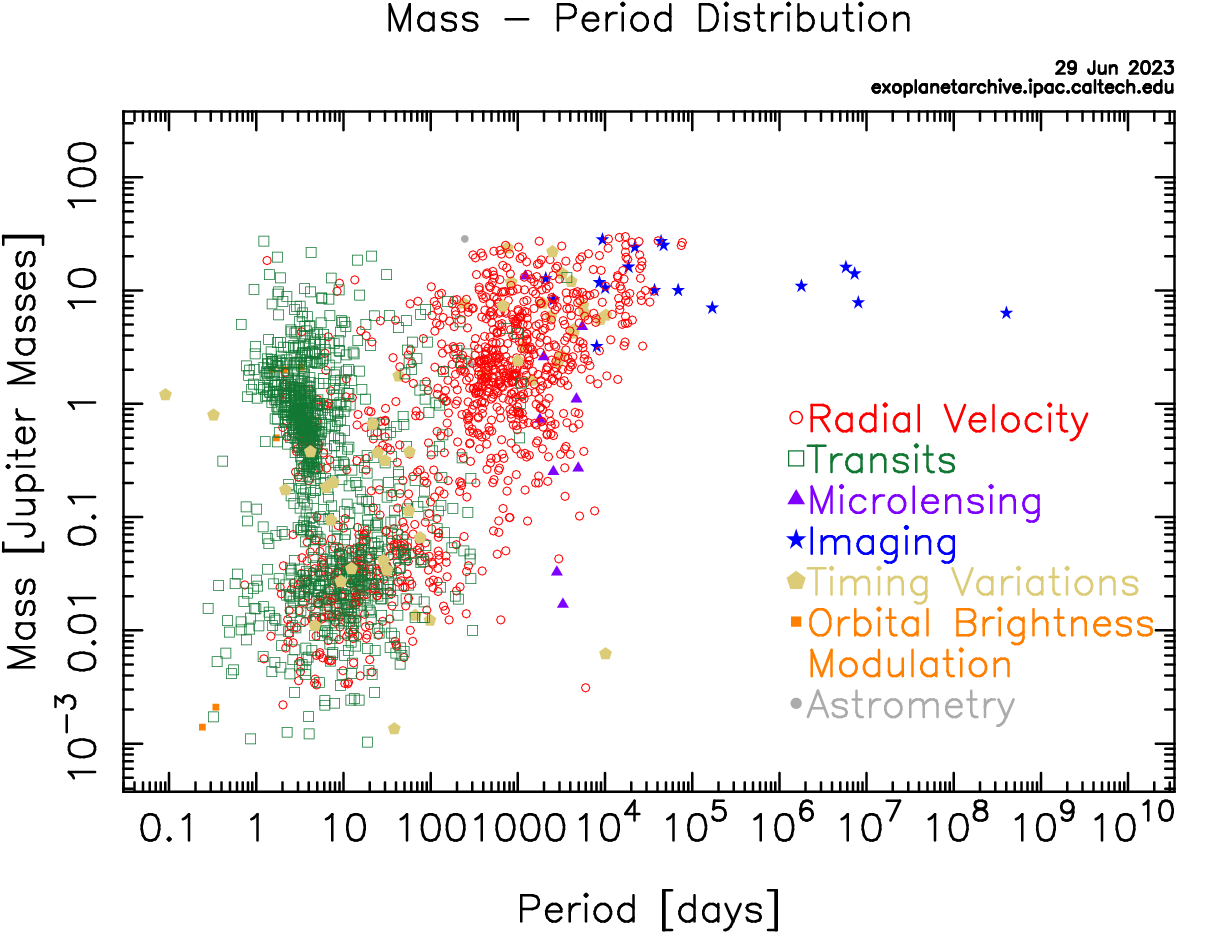
\includegraphics[width=0.95\textwidth]{intro/exo_massperiod.png}
  \end{center}
  \caption{The mass-period distribution of known exoplanets on the 
  NASA Exoplanet Archive on June 29th 2023
  \citep{akesonNASAExoplanet2013}. The plot is taken from the Archive
  itself which remakes the plot every time a planet is added.}
  \label{fig:archive_exoplanet_distribution}
\end{figure}

There are many different ways to detect an exoplanet, all of which provide
different information on the planet and are biased towards certain kinds of
planets. An easy way to see this is \Cref{fig:archive_exoplanet_distribution},
which plots all published exoplanets that have been added to the NASA Exoplanet
Archive, a database that contains the information on all published exoplanets,
at the time of writing in June 2023. Each detection method covers a different
range of periods and masses in the figure, representing the kinds of planet
planets the detection method is biased towards.

There are two broad forms of exoplanet detection, direct and indirect. Direct
detection of an exoplanet requires light to be collected from the planet itself
whereas indirect detection of an exoplanet is when the planet can be inferred
based on the star's light or circumstellar disk. The techniques that are
relevant to this work are direct imaging, radial velocity, transit photometry,
and astrometry. The transit technique has detected the most planets. Currently,
the NASA Exoplanet Archive has 4114 planets detected via transit, 1044 detected
via radial velocity, 67 detected with imaging, and 2 detected with astrometry.
These numbers are steadily increasing and missions such as TESS
\citep{Huang2018} and Gaia \citep{Perryman2018a} will increase the number of
known exoplanets by the thousands.

\subsection{Indirect Detection} 

The first unambiguous exoplanet detection around a Sun-like star occurred in
1995 through radial velocity observations of the star 51 Peg
\citep{mayorJupitermassCompanion1995}. The radial velocity method works by
observing the Doppler shift in a star's spectral lines and inferring the motion
of the star around a planet-star center of mass. This method is biased towards
massive planets on higher inclination orbits as the strength of a radial
velocity signal is determined by the factor $M\sin{i}$, where $M$ is the
planet's mass and $i$ is the inclination of the planet's orbit. The transit
photometry exoplanet detection technique finds planets by carefully monitoring
the light coming from stars and watching for dips that occur when a planet
passes in front of the star. The radius and orbital period of an exoplanet can
be determined with this technique and it is biased towards large radius planets
that are close to their star. The astrometry detection method involves
extremely precise measurements of a star's position in the plane of the sky
\citep{Perryman2018a}. With the precise movement of the star, the corresponding
motion of the planets can be inferred.


\subsection{Direct Detection}

Direct detection of exoplanets is the process of collecting light directly from
the exoplanet. This can be done when the planet is hot enough to emit light on
its own or when light from the star reflects off of the planet. Direct
detection is biased toward large radius planets at wide separations. Because of
this direct imaging complements the other techniques by broadening the range of
orbital periods that we are able to detect, as can be seen in the upper right
part of \Cref{fig:archive_exoplanet_distribution}. A further benefit of direct
imaging is its ability to obtain detailed spectral information on planets.
Gathering spectral information is of primary interest because it allows us to
study the atmosphere of the planet and search for signs of water and
biosignatures.

\section{Method Outlook}
\label{sec:EPRV_HWO}

This dissertation will focus on the synergy of using radial velocity data to
predict the best times to make observations of exoplanets with a direct imaging
instrument. This combination was chosen due to the extreme difficulty of
getting spectral information on Earth-like exoplanets. The 2020 decadal report
recommended a 6 meter space-based telescoped optimized for directly detecting
and spectrally characterizing habitable exoplanets
\citep{nationalacademiesofsciencesPathwaysDiscoveryAstronomy2021} based on the
HabEx and LUVOIR mission concept studies
\citep{gaudiHabitableExoplanetObservatory2020,TheLUVOIRTeam2019}. Both the
HabEx and LUVOIR teams recommended considerable effort be put into finding
habitable worlds through other detection methods before the launch of a
space-based direct imaging mission. The main reason for this is simply that it
is easier to detect a planet when you know approximately where it will be.
Additionally, if a star is observed and no Earth-like planet is found then that
star can be removed from the direct imaging mission's list of stars to observe,
or target list. 

Earth-like planets around Sun-like stars are difficult to detect for any
method. They have a very low probability of transiting, astrometric detection
of an Earth-like planet can only be done with a space-based mission two orders
of magnitude more sensitive than the Gaia mission, and the radial velocity
method requires sensitivity improvements between one and two orders of
magnitude (depending on what instrument is considered a baseline sensitivity)
to detect an Earth-like planet \citep{gaudiHabitableExoplanetObservatory2020}.
However, the radial velocity method can feasibly make the required improvements
with ground based observatories and many efforts to reach the required
sensitivity are in progress\citep{Fischer2016a}. The radial velocity precision
required to detect an Earth-like planet is approximately 10 cm/s and a number
of instruments have recently demonstrated on-sky radial velocity precision
under 1 m/s \citep{maroonx2021, guptaTargetPrioritization2021,Pepe2021}.
Additionally, the 2021 Extreme Precision Radial Velocity initiative report
concluded that there are multiple, plausible system architectures that can
detect Earth-like exoplanets under the right conditions \citep{Crass2021}.

\section{Yield modeling}
\label{sec:intro_yield_modeling}

In studying future missions, an early step is to have some estimate of what
kind of science can be accomplished by the mission. This leads to the idea of
``yield modeling'', methods that can compare different mission designs to
determine a trade space between cost and what kind of science a mission can do.
For exoplanet direct imaging, yield is typically treated as the number of
planets that can be detected
\citep{brownSingleVisitPhotometric2005,savranskyAnalyzingDesignsPlanetFinding2010,
starkMaximizingExoEarthCandidate2014}. Yield modeling plays an important role
in the mission design process and studies have looked at how different
mission components impact exoplanet yield: precursor knowledge
\citep{morganFasterExoEarth2021}, the starlight suppression system
\citep{savranskyAnalyzingDesignsPlanetFinding2010,morgan19, Stark2016},
aperture size \citep{starkLowerLimitsAperture2015}, planet population
\citep{savranskyComparisonAnalyticalDepth2016}, and more. 

It is impossible to separate the work of exoplanet observation scheduling and
the science yield of an exoplanet mission. When simulating a mission to
establish the number of planets that can be detected there must be some choices
made to determine what order stars are observed in. The trade space is
effectively: what star should be observed, at what time, and for how long. Because
direct imaging depends on reflected light (for most planets) there are usually
considerable portions of an exoplanet's orbit when it is not detectable so the
choice of when to observe a star is vital to whether an exoplanet is detected.
Without simulating the process of observation scheduling in full it cannot be
proven that a mission will be able to make observations at the most
advantageous times for all target stars. In this manner yield modeling and
observation scheduling are inherently linked and important for mission design.


\section{Dissertation Overview}
\label{sec:dis_overview}

In this dissertation, I present my contributions to improve our chances of
directly imaging an exoplanet that has been detected with the radial velocity
method. In \Cref{cha:first_paper} I begin by analyzing what orbital information
is missing from a radial velocity fit, how to fill the information, how to use
that information to estimate the probability of a telescope directly detecting
that planet, and what can go wrong when doing so. My contributions on this
topic come from my analysis of using orbital fit information to predict the
probability of detection and the two failure modes that can occur. The work of
\Cref{cha:first_paper} was published as \citet{spohnSchedulingDirect2022}. Then
in \Cref{cha:coupling} I describe a method to accurately estimate what the
dimmest planet a direct imaging mission can detect in the likely scenario where
the planet's brightness has a subtle impact on the amount of observational
noise. The work of \Cref{cha:coupling} was published in the paper
\citet{spohnDirectImaging2022} and is incorporated in the Imaging Mission
Database's \citep{savranskyExplorationDynamical2019} estimates of observing
mode specific completeness. The methods of \Cref{cha:coupling} are combined
with the probability of detection metric from \Cref{cha:first_paper} in
\Cref{cha:accurate_pdet} to calculate the probability of detection method with
more factors to describe more realistic observation scenarios. It is the first
method of calculating the probability of direct imaging detection as a function
of observation time and integration time for planets with precursor radial
velocity information. Then in \Cref{cha:sim_and_scheduling}, I validate the
probability of detection calculations with a software tool I created that
manages the creation of synthetic planetary systems, the radial velocity
observation process on the synthetic planetary systems, full orbital fitting of
the collected radial velocity data, calculating the probability of detecting
the synthetic planets that were fitted, scheduling observations based on the
probability of detection, and finally simulating direct imaging observations
based on the created schedule to determine its yield. The work in
\Cref{cha:sim_and_scheduling} is the first direct imaging mission scheduler to
simulate the collection and use of precursor data and is the first application
of constraint programming to the problem of direct imaging observation
scheduling.
